\section{Durchführung}
\label{sec:Durchführung}

Der Versuch wird an einem System an Strömungsrohren durchgeführt, welche mit einem
Gemisch aus Wasser, Glycerin und Glaskugeln gefüllt sind. Die Flussgeschwindigkeit
dieses Gemischs kann mithilfe einer in das System integrierten Zentrifugalpumpe geregelt werden.

\begin{figure}[H]
  \centering
  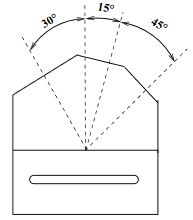
\includegraphics[height=5cm]{Prisma.PNG}
  \caption{Abbildung eines Doppler-Prismas. \cite{sample}}
  \label{fig:prisma}
\end{figure}

Zu Beginn werden Doppler-Prismen (Abbildung \ref{fig:prisma}) auf drei zu untersuchende Schlauchstellen gesteckt.
Dabei wird auf die Prismen an ihrer Kontaktstelle zum Schlauch sowie oben auf die
späteren Kontaktstellen zur Ultraschallsonde jeweils Ultraschallgel aufgetragen, um
die Messung vernünftig durchführen zu können. Sodann wird eine Ultraschallsonde an einen
Doppler-Generator angeschlossen. Dieser ist ebenfalls mit einem Rechner verbunden,
auf dem die Ergebnisse der Messung dargestellt werden können.

Anschließend werden dann jeweils an allen drei Einstellflächen  (15°, 30°, 60°) eines jeden Prismas
(welche sich an den drei unterschiedlich dicken zu untersuchenden Rohren befinden)
für fünf unterschiedliche Strömungsgeschwindigkeiten die Frequenzverschiebungen gemessen.

Im zweiten Teil des Versuchs wird dann ein Strömungsprofil der Dopplerflüssigkeit erstellt.
Dazu wird bei insgesamt zwei verschiedenen Strömungsgeschwindigkeiten in unterschiedlichen
Tiefen des Rohres die Frequenzänderung sowie die Standardabweichung bestimmt.
Die Messtiefe kann dabei am Ultraschallgenerator eingestellt werden.
